
% Apache Hive Seminar - Condensed 6-Slide Version
\documentclass[aspectratio=169,10pt]{beamer}
\usetheme{Madrid}
\usecolortheme{whale}
\definecolor{africanblue}{RGB}{0, 102, 153}
\definecolor{earthgreen}{RGB}{34, 139, 34}
\definecolor{oceanblue}{RGB}{0, 119, 182}
\definecolor{sunsetorange}{RGB}{230, 126, 34}
\setbeamercolor{structure}{fg=africanblue}
\setbeamercolor{frametitle}{bg=africanblue!90,fg=white}
\setbeamercolor{title}{fg=white,bg=africanblue}
\setbeamercolor{block title}{bg=oceanblue,fg=white}
\setbeamercolor{block body}{bg=oceanblue!10}
\setbeamercolor{item}{fg=earthgreen}
\setbeamercolor{block title example}{bg=earthgreen!80,fg=white}
\setbeamercolor{block body example}{bg=earthgreen!10}
\setbeamercolor{block title alerted}{bg=red!70,fg=white}
\setbeamercolor{block body alerted}{bg=red!10}
\usepackage{tikz}
\usetikzlibrary{shapes,arrows,positioning,calc,fit,backgrounds}
\usepackage{fontawesome5}
\usepackage{booktabs}
\usepackage{graphicx}
\usepackage{listings}
\usepackage{xcolor}
\usepackage{hyperref}
\setbeamerfont{itemize/enumerate body}{size=\small}
\setbeamerfont{itemize/enumerate subbody}{size=\footnotesize}
\setbeamerfont{block body}{size=\small}
\lstset{
    basicstyle=\tiny\ttfamily,
    backgroundcolor=\color{gray!10},
    frame=single,
    breaklines=true,
    keywordstyle=\color{blue},
    commentstyle=\color{earthgreen},
    stringstyle=\color{sunsetorange}
}
\title[Apache Hive Seminar]{\textbf{Apache Hive: Architecture, Optimization, and Experimental Validation}}
\subtitle{MBV Climate and Ocean Intelligence Africa}
\author{Dushime Mudahera Richard}
\institute{Databases for Big Data Seminar -- Prof.\ Iztok Savnik}
\date{January 2026}
\setbeamertemplate{navigation symbols}{}
\setbeamertemplate{footline}[frame number]
\begin{document}

% SLIDE 1: TITLE
\begin{frame}[plain]
    \titlepage
    \begin{tikzpicture}[remember picture,overlay]
        \node[opacity=0.1] at (current page.center) {\scalebox{8}{\faCloud}};
    \end{tikzpicture}
\end{frame}

% SLIDE 2: OVERVIEW & OBJECTIVES
\begin{frame}{Overview \& Objectives}
    \begin{block}{Context}
        \textbf{Apache Hive} is a data warehouse system built on Hadoop, providing SQL-like analytics at petabyte scale. This work analyzes its architecture, storage, optimization, and validates with real execution logs.
    \end{block}
    \vspace{0.2cm}
    \begin{block}{Objectives}
        \begin{enumerate}
            \item Analyze Hive's architecture and core components
            \item Explain query compilation and execution
            \item Evaluate storage model: partitions, buckets, schema-on-read
            \item Assess optimization: CBO, join strategies
            \item Validate with log-based experimentation
        \end{enumerate}
    \end{block}
\end{frame}

% SLIDE 3: ARCHITECTURE & PIPELINE
\begin{frame}{System Architecture \& Query Pipeline}
    \begin{columns}[T]
        \column{0.55\textwidth}
        \begin{block}{Core Components}
            \begin{itemize}
                \item \textbf{Driver}: Orchestrates session, submits queries
                \item \textbf{Compiler}: Parses, plans, and optimizes queries
                \item \textbf{Metastore}: Schema-on-read, stores table/partition metadata (PostgreSQL backend)
                \item \textbf{Execution Engine}: MapReduce (MR) jobs
                \item \textbf{HDFS}: Distributed storage
            \end{itemize}
        \end{block}
        \vspace{0.2cm}
        \begin{block}{Query Compilation Pipeline}
            \begin{enumerate}
                \item Parse (ANTLR $\to$ AST)
                \item Semantic Analysis (Metastore lookup)
                \item Logical Plan (operator tree)
                \item Optimization (Calcite CBO)
                \item Physical Plan (MR stages)
            \end{enumerate}
        \end{block}
        \column{0.45\textwidth}
        \begin{center}
            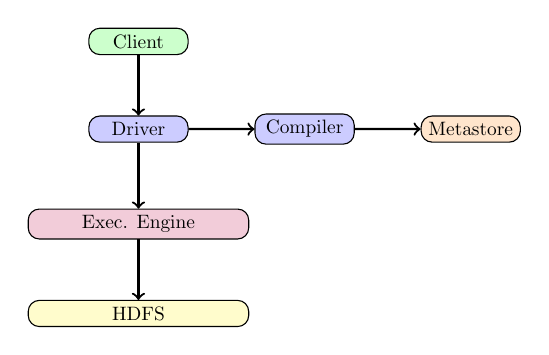
\begin{tikzpicture}[node distance=1.1cm, scale=0.7, transform shape]
                \node[draw,rounded corners,fill=green!20,minimum width=1.8cm] (client) {Client};
                \node[draw,rounded corners,fill=blue!20,below=of client,minimum width=1.8cm] (driver) {Driver};
                \node[draw,rounded corners,fill=blue!20,right=1.2cm of driver,minimum width=1.8cm] (compiler) {Compiler};
                \node[draw,rounded corners,fill=orange!20,right=1.2cm of compiler,minimum width=1.8cm] (meta) {Metastore};
                \node[draw,rounded corners,fill=purple!20,below=1.2cm of driver,minimum width=4cm] (engine) {Exec. Engine};
                \node[draw,rounded corners,fill=yellow!20,below=of engine,minimum width=4cm] (hdfs) {HDFS};
                \draw[->,thick] (client) -- (driver);
                \draw[->,thick] (driver) -- (compiler);
                \draw[->,thick] (compiler) -- (meta);
                \draw[->,thick] (driver) -- (engine);
                \draw[->,thick] (engine) -- (hdfs);
            \end{tikzpicture}
        \end{center}
    \end{columns}
\end{frame}

% SLIDE 4: STORAGE MODEL & OPTIMIZATIONS
\begin{frame}{Storage Model \& Optimizations}
    \begin{columns}[T]
        \column{0.5\textwidth}
        \begin{block}{Storage Model}
            \begin{itemize}
                \item \textbf{Databases, Tables}: Managed vs. External
                \item \textbf{Partitions}: Directory-based, enables pruning
                \item \textbf{Buckets}: Hash-based, enables SMB joins
                \item \textbf{Schema-on-Read}: Structure applied at query time
                \item \textbf{ORC+SNAPPY}: Columnar, compressed
            \end{itemize}
        \end{block}
        \column{0.5\textwidth}
        \begin{block}{Optimization Techniques}
            \begin{itemize}
                \item \textbf{Partition Pruning}: Skip irrelevant data
                \item \textbf{Bucketing}: Enables efficient joins
                \item \textbf{Vectorized Execution}: 1,024 rows/instruction
                \item \textbf{CBO (Calcite)}: Cost-based plan selection
                \item \textbf{Map-Side Join}: Broadcast small tables
            \end{itemize}
        \end{block}
    \end{columns}
\end{frame}

% SLIDE 5: EXPERIMENTAL VALIDATION (LOGS)
\begin{frame}{Experimental Validation: Log Analysis}
    \begin{block}{Setup}
        7-container Docker stack: HiveServer2, Metastore (PostgreSQL), HDFS (1 NameNode, 2 DataNodes). Dataset: 4.75M climate records, 5,000 stations.
    \end{block}
    \vspace{0.2cm}
    \begin{block}{Execution Trace: Multi-Stage Query}
        \begin{itemize}
            \item \textbf{5 MapReduce Jobs:} Scan/Partial Agg $\to$ Shuffle/Reduce $\to$ Derived Computation $\to$ Global Sort $\to$ Result Materialization
            \item \textbf{Blocking:} Each stage waits for previous to finish (MR engine)
            \item \textbf{Map-Side Join:} Small table broadcast, 0 reducers, no shuffle
        \end{itemize}
    \end{block}
    \begin{block}{Performance}
        Map-Side Join: \textbf{15.3s}, Reduce-Side Join: \textbf{42.7s} (2.8x speedup). ORC: \textbf{88\%} compression. Query latency: 9--26s.
    \end{block}
\end{frame}

% SLIDE 6: CONCLUSION & TAKEAWAYS
\begin{frame}{Conclusion \& Takeaways}
    \begin{block}{Key Points}
        \begin{itemize}
            \item Hive abstracts MapReduce, but inherits disk I/O latency
            \item Schema-on-Read and partitioning enable scalable analytics
            \item CBO and join selection are critical for performance
            \item Log-based validation confirms theory: Map-Side Join, partition pruning, and ORC yield major speedups
        \end{itemize}
    \end{block}
    \vspace{0.2cm}
    \begin{block}{Future Work}
        Migrate to Tez or Spark to reduce intermediate I/O bottlenecks and enable pipelined execution.
    \end{block}
    \vspace{0.2cm}
    \centering{\small \textbf{Dushime Mudahera Richard} -- Databases for Big Data Seminar, January 2026}
\end{frame}

\end{document}